\documentclass{layout/epfl-report}
\usepackage{csquotes}

%% Configuración de la bibliografía
\usepackage[spanish]{babel} % Idioma español
\usepackage{svg}
\usepackage{pdflscape}
\usepackage{listings}

% Configuración básica
\lstset{
  basicstyle=\ttfamily\small, % Estilo básico del texto
  frame=single, % Marco alrededor del código
  backgroundcolor=\color{gray!10}, % Fondo gris claro
  keywordstyle=\bfseries\color{blue}, % Palabras clave en azul
  breaklines=true, % Divide líneas largas automáticamente
  columns=flexible % Ajusta el espaciado entre caracteres
}

\usepackage{biblatex}
%\addbibresource{report.bib}
\addbibresource{references/chapter-1.bib}
%\addbibresource{chapter-2.bib}
%\addbibresource{chapter-3.bib}
%\addbibresource{chapter-4.bib}
%\addbibresource{chapter-5.bib}
%\addbibresource{chapter-6.bib}
%\addbibresource{chapter-7.bib}
%\addbibresource{chapter-8.bib}
%\addbibresource{chapter-9.bib}
%\addbibresource{chapter-10.bib}

%% Paquetes adicionales y comandos
\usepackage{graphicx}
\setlist{itemsep=-2pt} % Reducir el espacio en listas
\renewcommand{\deg}{\si{\degree}\xspace} % Usar \deg fácilmente

%% ----------------------------------------------------------------------
%%    Inicio del documento + Portada (Numeración romana)
%% ----------------------------------------------------------------------

\begin{document}

\frontmatter

%% Definición de parámetros principales
\title{Consideraciones éticas en el desarrollo e implementación de tecnologías emergentes basadas en IA}
%\subtitle{Explorando dilemas éticos}
%\author{Nombre del Autor}

\subject{Grupo de Estudio: Ética en Tecnologías Emergentes Basadas en AI} % Solo para la portada
%\affiliation{Ecole Polytechnique Fédérale de Lausanne (EPFL)} % Solo para la portada
\coverimage{figures/cover8} % Relación de aspecto 2:3 (retrato) recomendada
\definecolor{title}{HTML}{FF6600} % Color para el título de la portada (naranja brillante)


\makecover

\begin{titlepage}

\begin{center}

%% Print the title
{\makeatletter
\largetitlestyle\fontsize{45}{45}\selectfont\@title
\makeatother}

%% Print the subtitle
{\makeatletter
\ifdefvoid{\@subtitle}{}{\bigskip\titlestyle\fontsize{16}{14}\selectfont\@subtitle}
\makeatother}

\bigskip
\bigskip

%by

\bigskip
\bigskip

%% Print the name of the author
%{\makeatletter
%\largetitlestyle\fontsize{25}{25}\selectfont\@author
%\makeatother}

\bigskip
\bigskip

%% Print table with names and student numbers
\setlength\extrarowheight{2pt}
%\begin{tabular}{lc}
%    Student Name & Student Number \\\midrule
%    First Surname & 123456 \\
%\end{tabular}

\vfill

%% Print some more information at the bottom
%\begin{tabular}{ll}
%    Instructor: & I. Surname \\
%    Teaching Assistant: & I. Surname \\
%    Project Duration: & Month, Year - Month, Year \\
%    Faculty: & School of Computer and Communication Sciences, EPFL
%\end{tabular}

\bigskip
\bigskip

%% Add a source and description for the cover and optional attribution for the template
\begin{tabular}{p{15mm}p{10cm}}
%    Cover: & The Rolex Learning Center at EPFL (Modified) \\
    % Feel free to remove the following attribution, it is not required - still appreciated :-)
   % Style: & EPFL Report Style, with modifications by Batuhan Faik Derinbay
\end{tabular}

\end{center}

%% Insert the EPFL logo at the bottom of the page
%\begin{tikzpicture}[remember picture, overlay]
%    \node[above=10mm] at (current page.south) {%
%         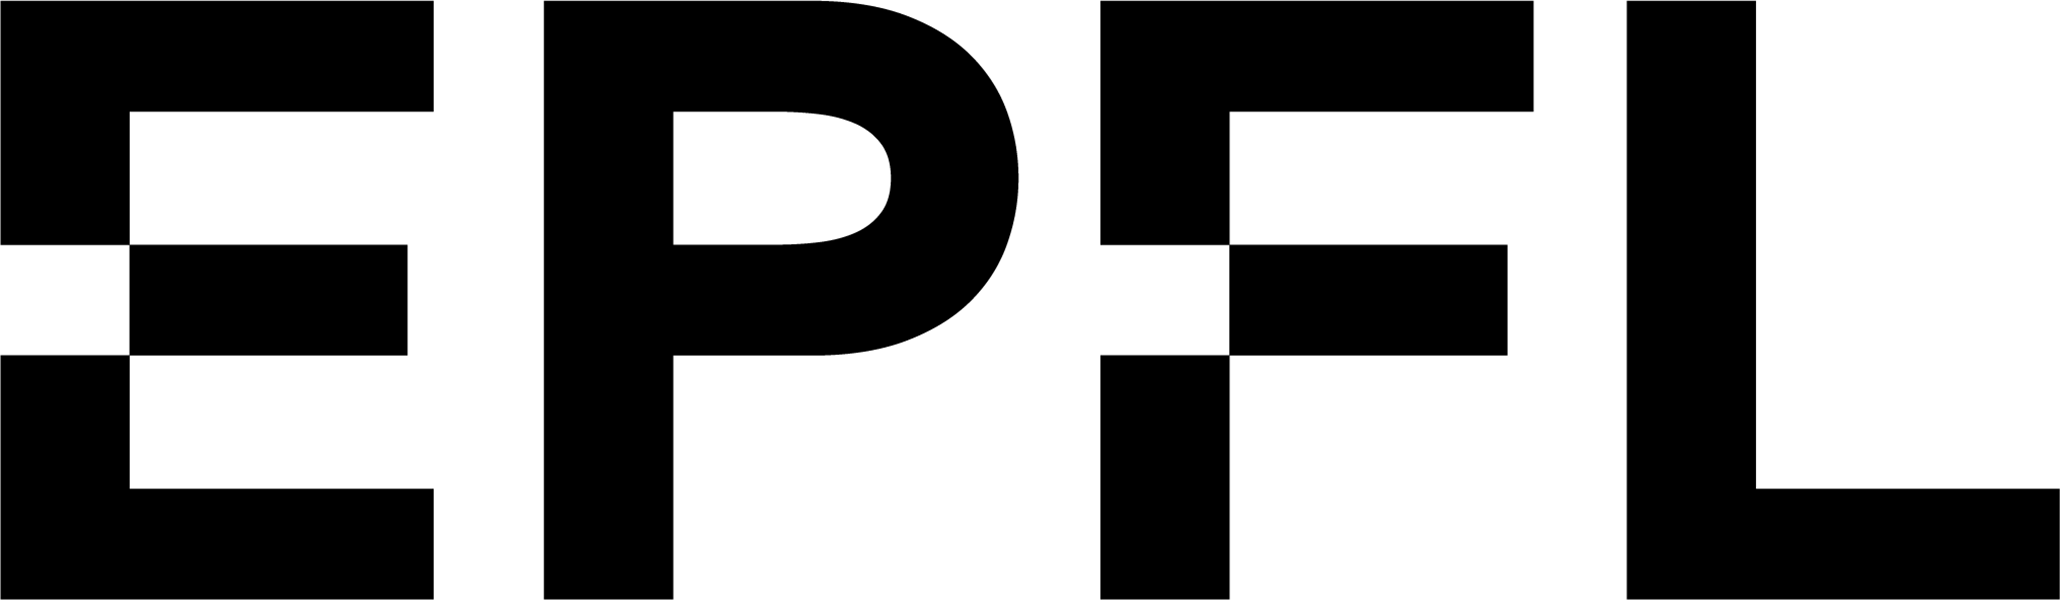
\includegraphics[width=0.35\linewidth]{layout/epfl/logo-black}
%    };
%\end{tikzpicture}

\end{titlepage}

%\chapter*{Preface}
\addcontentsline{toc}{chapter}{Preface}

\emph{A preface...}

\begin{flushright}
{\makeatletter\itshape
    \@author \\
    EPFL, \monthname{} \the\year{}
\makeatother}
\end{flushright}

\chapter*{Resumen}
\addcontentsline{toc}{chapter}{Resumen}

\emph{Este documento de trabajo está diseñado como una guía comprensiva para estudiar y reflexionar sobre los desafíos éticos en el desarrollo y aplicación de tecnologías emergentes basadas en inteligencia artificial (IA) con un enfoque en Python como herramienta principal.}

En un mundo donde las tecnologías avanzadas están remodelando las estructuras sociales, económicas y ambientales, es fundamental examinar no solo los beneficios, sino también las implicaciones éticas que conllevan. Este documento aborda de manera estructurada una serie de temas clave, organizados en 20 capítulos, que exploran aspectos críticos de la ética en IA y tecnologías emergentes:

\begin{itemize}
    \item **Impacto social y ambiental:** Reflexión sobre cómo las tecnologías emergentes afectan la sociedad, desde la disrupción laboral hasta la sostenibilidad medioambiental.
    \item **Explicabilidad e interpretabilidad:** Análisis de herramientas y metodologías para hacer que los sistemas de IA sean más transparentes y comprensibles.
    \item **Justicia algorítmica y sesgos:** Exploración de los riesgos asociados con decisiones algorítmicas injustas y cómo mitigarlos utilizando Python.
    \item **Gobernanza de AI  y privacidad:** Discusión sobre la soberanía digital, protección de datos y gobernanza ética en un mundo interconectado.
    \item **Innovación sostenible:** Evaluación de prácticas para equilibrar el desarrollo tecnológico con la sostenibilidad y los derechos humanos.
    \item **Reflexión filosófica:** Análisis de dilemas éticos y preguntas fundamentales como "¿Deberíamos hacerlo simplemente porque podemos?"
\end{itemize}

Cada capítulo combina teoría y práctica, proporcionando:
\begin{enumerate}
    \item Un marco conceptual que guía el análisis ético de los temas tratados.
    \item Ejercicios prácticos utilizando Python, para aplicar conceptos a casos del mundo real.
    \item Reflexiones críticas para fomentar un pensamiento ético informado y colaborativo.
\end{enumerate}

Este documento no solo busca equipar a los estudiantes y profesionales con herramientas técnicas y éticas, sino también fomentar un diálogo interdisciplinario sobre el futuro responsable de las tecnologías emergentes. Es un recurso dirigido a grupos de estudio, desarrolladores, investigadores y profesionales interesados en la intersección entre IA, ética y sostenibilidad, y destaca la importancia de Python como una plataforma poderosa para enfrentar estos desafíos de manera práctica.

\emph{La ética no es un obstáculo para la innovación, sino una brújula que nos guía hacia un progreso más inclusivo, justo y sostenible.}


\tableofcontents
%\listoffigures
%\listoftables

\chapter*{Nomenclatura}
\addcontentsline{toc}{chapter}{Nomenclatura}

\section*{Abreviaturas}

\begin{longtable}{p{3cm}p{9cm}}
    \toprule
    \textbf{Abreviatura} & \textbf{Definición} \\
    \midrule\endhead % Añadir abreviaturas aquí:
    \textbf{IA} & Inteligencia Artificial \\
    \textbf{LAWS} & \textit{Lethal Autonomous Weapon Systems} (Sistemas Autónomos Letales) \\
    \textbf{CRISPR} & \textit{Clustered Regularly Interspaced Short Palindromic Repeats} (Repeticiones Palindrómicas Cortas Agrupadas y Regularmente Interespaciadas) \\
    \textbf{IoT} & \textit{Internet of Things} (Internet de las Cosas) \\
    \textbf{FAIR} & \textit{Findable, Accessible, Interoperable, Reusable} (Localizable, Accesible, Interoperable, Reutilizable) \\
    \textbf{NLP} & \textit{Natural Language Processing} (Procesamiento de Lenguaje Natural) \\
    \textbf{DL} & \textit{Deep Learning} (Aprendizaje Profundo) \\
    \bottomrule
\end{longtable}

\section*{Símbolos}

\begin{longtable}{p{3cm}p{9cm}p{3cm}}
    \toprule
    \textbf{Símbolo} & \textbf{Definición} & \textbf{Unidad} \\
    \midrule\endhead % Añadir símbolos latinos aquí:
    $V$ & Velocidad & [m/s] \\
    $E$ & Energía & [J] \\
    $t$ & Tiempo & [s] \\
    \midrule % Añadir símbolos griegos aquí:
    $\rho$ & Densidad & [kg/m$^3$] \\
%    $\alpha$ & Ángulo o coeficiente de absorción & [-] \\
%    $\mu$ & Coeficiente de fricción & [-] \\
    \bottomrule
\end{longtable}

\section*{Glosario Técnico}

\begin{longtable}{p{3cm}p{9cm}}
    \toprule
    \textbf{Término} & \textbf{Definición} \\
    \midrule\endhead
    \textbf{Explicabilidad} & Capacidad de un modelo o sistema para proporcionar razones claras y comprensibles sobre cómo llegó a sus resultados. \\
    \textbf{Interpretabilidad} & Nivel al que un ser humano puede entender la causa detrás de una decisión tomada por un modelo. \\
    \textbf{Sesgo (Bias)} & Tendencia o parcialidad en un modelo de inteligencia artificial que puede llevar a resultados injustos o discriminatorios. \\
    \textbf{Sostenibilidad} & Uso responsable de recursos que asegura que las tecnologías no comprometan las necesidades de generaciones futuras. \\
    \textbf{Blockchain} & Tecnología de registro distribuido que asegura transparencia y seguridad en transacciones y datos digitales. \\
    \textbf{Transhumanismo} & Movimiento filosófico y científico que busca mejorar las capacidades humanas mediante el uso de tecnologías avanzadas. \\
    \textbf{IA Generativa} & Subcampo de la inteligencia artificial enfocado en crear contenido nuevo (imágenes, texto, música) basado en datos existentes. \\
    \textbf{Privacidad} & Derecho de los individuos a controlar el acceso a sus datos personales y su exposición en entornos digitales. \\
    \textbf{Riesgo Existencial} & Escenarios donde tecnologías emergentes podrían causar un daño irreversible a la humanidad o el ecosistema. \\
    \bottomrule
\end{longtable}


%% ----------------------------------------------------------------------
%%    Cuerpo del documento (Numeración arábiga)
%% ----------------------------------------------------------------------

\mainmatter

% Introducción en español

\begin{refsection}[references/chapter-1.bib]
\chapter{Introducción General}
\label{chapter:introduction_general}

\section{Propósito y Contexto}

Este capítulo introductorio tiene como objetivo presentar los principales desafíos éticos, sociales y técnicos asociados a las tecnologías emergentes, sirviendo como un marco para el análisis detallado que se desarrollará en los capítulos siguientes. A lo largo de este documento, exploraremos cómo la comunidad Python puede ser una fuerza impulsora para abordar estos desafíos de manera práctica, reflexiva y ética.


En este contexton, las tecnologías emergentes, como la inteligencia artificial (IA), la biotecnología, el blockchain y la computación cuántica, están transformando radicalmente la forma en que vivimos, trabajamos y nos relacionamos. Sin embargo, estas innovaciones traen consigo desafíos éticos, sociales y técnicos, por ejemplo:

\begin{itemize} \item \textbf{Desigualdad Tecnológica:}
El acceso desigual a tecnologías avanzadas perpetúa y amplifica las brechas económicas y sociales: \begin{itemize} \item Las comunidades marginadas tienen menos acceso a los beneficios tecnológicos. \item Las plataformas globales, diseñadas por y para sectores privilegiados, generan exclusión digital. \end{itemize}

\item \textbf{Impacto de la Centralización Tecnológica:}  
La creciente concentración de recursos computacionales y tecnológicos en unas pocas entidades globales plantea serios riesgos para la equidad:
\begin{itemize}
    \item Los monopolios tecnológicos limitan la innovación local y el control soberano sobre infraestructuras clave.
    \item La dependencia de servicios de almacenamiento y cómputo en la nube controlados por corporaciones globales afecta la soberanía digital de países en desarrollo.
\end{itemize}

\item \textbf{Justicia Algorítmica:}  
Los sistemas basados en IA pueden perpetuar y amplificar desigualdades estructurales existentes:
\begin{itemize}
    \item Algoritmos de contratación, sistemas judiciales y modelos de evaluación educativa han demostrado sesgos hacia comunidades desfavorecidas.
    \item La falta de transparencia en modelos de aprendizaje profundo dificulta auditar y corregir estos sesgos.
\end{itemize}

\item \textbf{Soberanía Digital:}  
El control global sobre tecnologías e infraestructuras digitales por parte de pocas corporaciones amenaza la autonomía local:
\begin{itemize}
    \item Las comunidades pierden control sobre sus datos y recursos tecnológicos.
    \item Modelos descentralizados, como blockchain, ofrecen alternativas, pero necesitan regulación ética para evitar la concentración de poder.
\end{itemize}

\item \textbf{Secuencias Genéticas Digitalizadas y Biopiratería:}  
La digitalización de recursos genéticos plantea serios desafíos éticos y legales:
\begin{itemize}
    \item Los vacíos en los Protocolos de Nagoya permiten el uso no regulado de secuencias genéticas digitalizadas.
    \item Las comunidades indígenas no reciben beneficios por el conocimiento tradicional asociado a estos recursos.
    \item Es crucial implementar tecnologías como blockchain para rastrear el uso de recursos genéticos y garantizar una distribución justa de beneficios.
\end{itemize}

\item \textbf{Manipulación Genética y Ética Biotecnológica:}  
La edición genética y el biohacking plantean nuevas preguntas sobre los límites éticos de la intervención humana en la biología:
\begin{itemize}
    \item La modificación genética en humanos podría exacerbar desigualdades o ser utilizada para propósitos eugenésicos.
    \item Aplicaciones no terapéuticas de la biotecnología, como el biohacking, carecen de marcos regulatorios claros.
\end{itemize}

\item \textbf{Computación Cuántica y Seguridad Global:}  
Las capacidades disruptivas de la computación cuántica presentan riesgos significativos para la seguridad digital:
\begin{itemize}
    \item Sistemas actuales de criptografía pueden quedar obsoletos, exponiendo datos sensibles.
    \item Es necesario desarrollar estándares globales de criptografía post-cuántica para proteger infraestructuras críticas.
\end{itemize}

\item \textbf{Privacidad y Ética del IoT e Inteligencia Ambiental:}  
La expansión de dispositivos conectados y entornos inteligentes plantea riesgos significativos para la privacidad y la autonomía individual:
\begin{itemize}
    \item La vigilancia masiva y la recopilación de datos personales crean una sociedad de control invisible.
    \item Los entornos inteligentes podrían manipular comportamientos de manera no ética, afectando especialmente a poblaciones vulnerables.
\end{itemize}

\item \textbf{Riesgos Existenciales de la IA General y Sistemas Autónomos:}  
La carrera por desarrollar inteligencia artificial general (AGI) y sistemas autónomos plantea riesgos globales significativos:
\begin{itemize}
    \item Drones autónomos y armas letales autónomas (LAWS) podrían desestabilizar equilibrios internacionales.
    \item La falta de gobernanza ética en AGI podría generar consecuencias catastróficas.
\end{itemize}

\item \textbf{Ética en el Metaverso:}  
Las economías y comunidades virtuales del metaverso introducen nuevos desafíos éticos y sociales:
\begin{itemize}
    \item La privacidad y el control de datos personales en entornos virtuales inmersivos necesitan mayor regulación.
\end{itemize}

\item \textbf{Eficiencia Energética y Computación Verde:}  
El crecimiento de tecnologías avanzadas requiere un replanteamiento de la eficiencia energética:
\begin{itemize}
    \item Diseñar sistemas que optimicen recursos energéticos puede reducir los costos operativos y la dependencia de infraestructuras intensivas en recursos.
    \item Soluciones como el \textit{edge computing} y la computación neuromórfica ofrecen alternativas para mitigar la centralización tecnológica.
\end{itemize}
\end{itemize}





\section{Metodología para la Identificación de Tópicos}

Para determinar los capítulos de este documento, se utilizó una metodología basada en análisis bibliométrico, técnicas de procesamiento de lenguaje natural (NLP) y algoritmos de detección de comunidades. Este enfoque combina herramientas técnicas avanzadas y contribuciones interdisciplinarias, permitiendo una síntesis integral de los temas más relevantes. El proceso se desarrolló en las siguientes etapas:

\subsection{Recopilación del Corpus Bibliográfico}

Se realizó una búsqueda en la base de datos Web of Science Core Collection utilizando la siguiente ecuación de búsqueda:

% Uso en el documento
\begin{lstlisting}[language=Python, caption={Ecuación de búsqueda en Web of Science}]
ALL=("ethics" AND ("artificial intelligence" OR "AI") AND 
("emerging technologies" OR "cutting-edge technologies") AND 
("frameworks" OR "dilemmas" OR "challenges" OR "policy"))
Refined By: Publication Years: 2024 OR 2023 OR 2022 OR 2021 OR 2020 
AND Open Access
\end{lstlisting}

\textbf{Resultados de la búsqueda:}

\begin{itemize}
    \item La búsqueda se realizó en la base de datos \textbf{Web of Science Core Collection}.
    \item \textbf{Número de resultados:} Se identificaron \textbf{45 publicaciones relevantes}.
    \item \textbf{Filtros aplicados:}
    \begin{itemize}
        \item Años de publicación: Entre \textbf{2020 y 2024}.
        \item \textbf{Acceso abierto:} Solo se incluyeron artículos de acceso abierto para garantizar accesibilidad.
    \end{itemize}
\end{itemize}

\textbf{Descripción del corpus bibliográfico:}

El corpus incluye artículos relacionados con los siguientes términos clave:
\begin{itemize}
    \item Ética aplicada a la IA y tecnologías emergentes.
    \item Marcos regulatorios, dilemas éticos y desafíos asociados al desarrollo de tecnologías de vanguardia.
    \item Políticas tecnológicas orientadas a la sostenibilidad, la justicia social y la gobernanza.
\end{itemize}

\textbf{Siguientes pasos:}
\begin{itemize}
    \item Construcción de un grafo de co-ocurrencia basado en las palabras clave y términos frecuentes.
    \item Análisis de comunidades temáticas utilizando el algoritmo de \textit{Modularity}.
    \item Síntesis de los tópicos más relevantes para determinar los capítulos del documento.
\end{itemize}


Los resultados fueron refinados para incluir únicamente publicaciones de acceso abierto de los años 2020 a 2024, obteniendo un total de 45 artículos relevantes. Estos artículos constituyen la base del análisis bibliométrico.

\subsection{Construcción del Grafo de Citas y Palabras Clave}

A partir del corpus bibliográfico, se construyó un grafo de co-ocurrencia utilizando técnicas de procesamiento de lenguaje natural (NLP):
\begin{itemize}
    \item \textbf{Extracción de términos clave:} Se analizaron títulos, resúmenes y palabras clave para identificar conceptos recurrentes.
    \item \textbf{Representación del grafo:} Cada nodo representa un término o concepto, y los enlaces indican la frecuencia de co-ocurrencia entre términos dentro del mismo documento.
    \item \textbf{Visualización del grafo:} El grafo se visualizó utilizando bibliotecas como \texttt{NetworkX} y \texttt{Gephi}, facilitando la interpretación de relaciones entre términos.
\end{itemize}

\subsection{Aplicación del Algoritmo de Modularity}

Para identificar comunidades temáticas emergentes dentro del grafo, se realizaron los siguientes pasos:
\begin{itemize}
    \item \textbf{Detección de comunidades:} Se utilizó el algoritmo de Modularity, optimizando la partición del grafo y agrupando términos relacionados en comunidades cohesivas.
    \item \textbf{Identificación de áreas temáticas:} Se detectaron un total de \textbf{117 comunidades emergentes}, cada una representando un área temática específica dentro del corpus bibliográfico.
    \item \textbf{Visualización del grafo:} La estructura resultante del grafo fue representada utilizando una herramienta de visualización que permite resaltar las comunidades temáticas.
\end{itemize}

\begin{landscape}
\begin{figure}[ht]
    \centering
    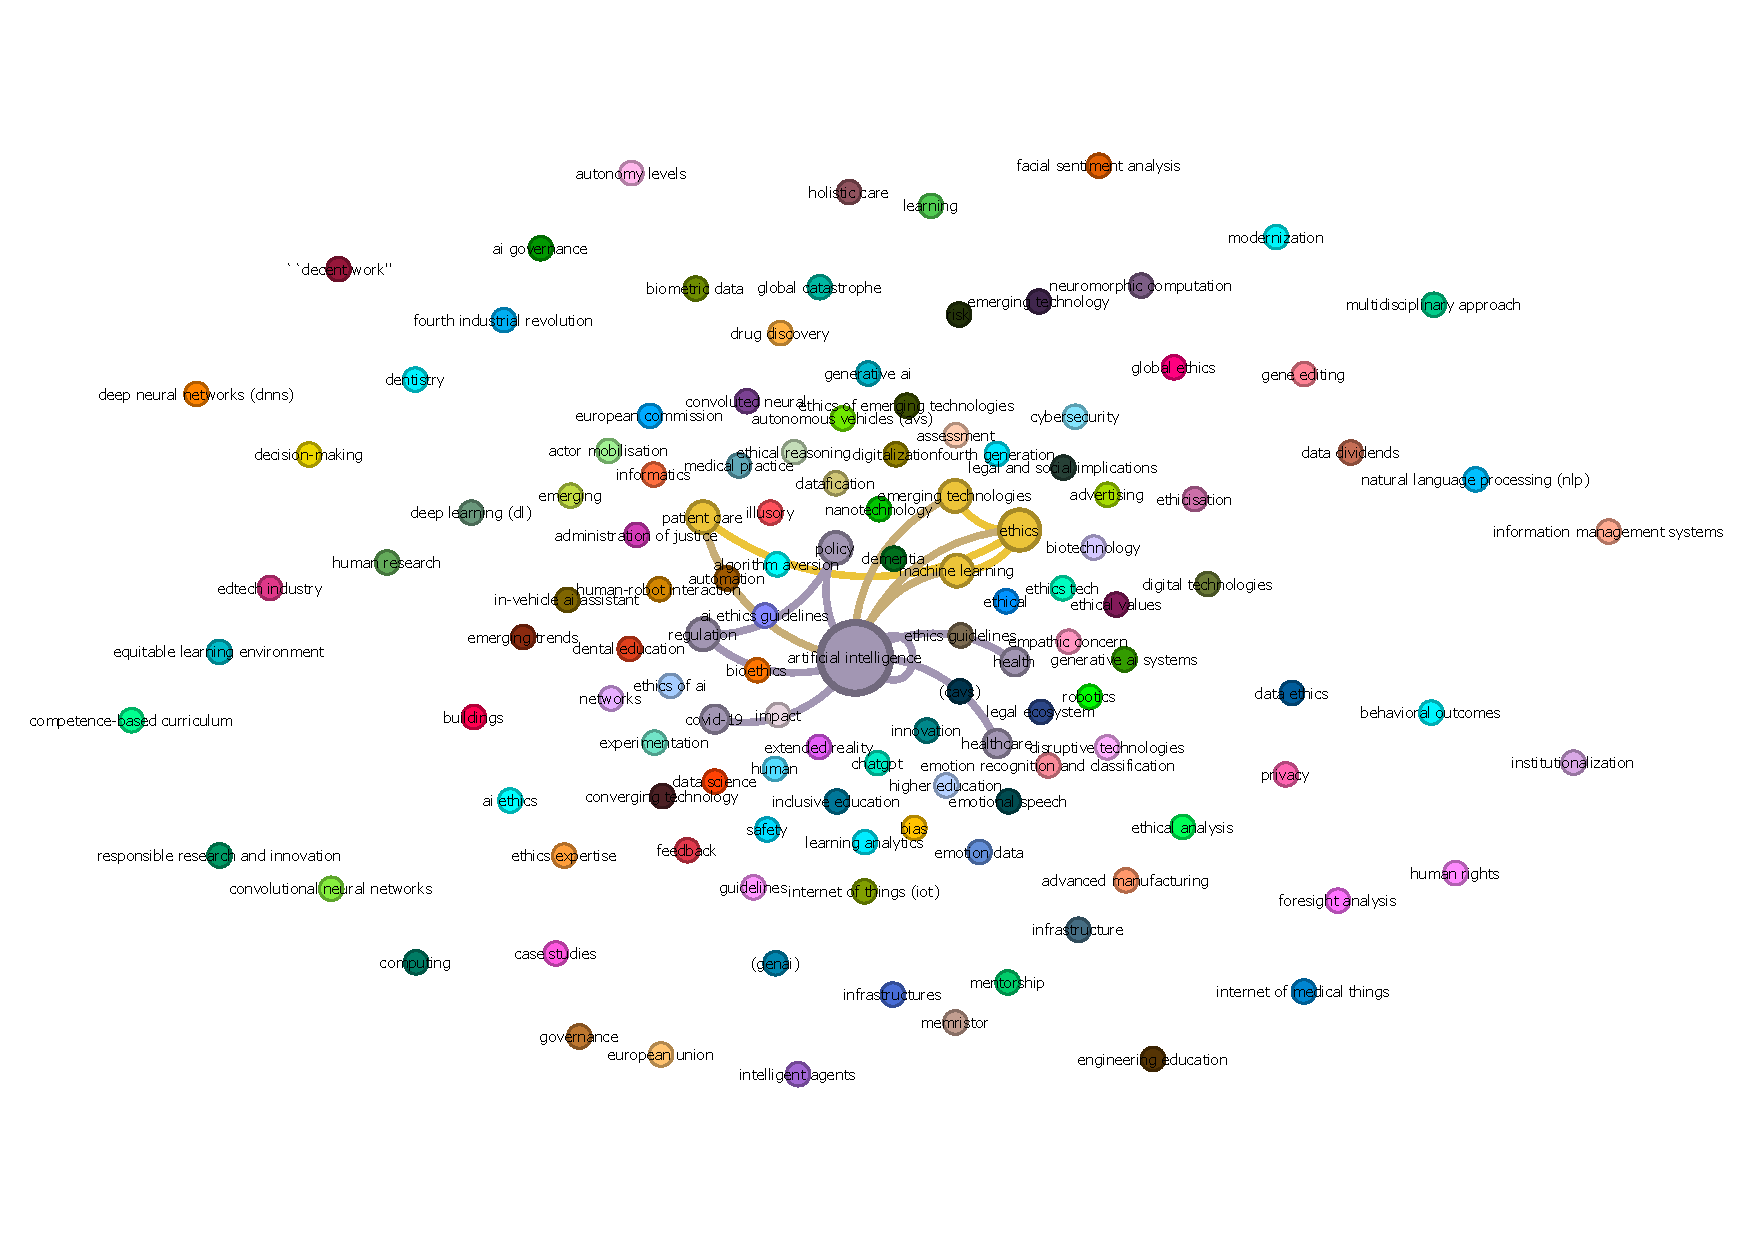
\includegraphics[width=1.5\textwidth, height=1\textheight, keepaspectratio=false]{figures/ethics_ai_emergent_tecnologies.pdf}
    \caption{Visualización del grafo de comunidades temáticas detectadas mediante el algoritmo de Modularity. Cada nodo representa un término, y las conexiones indican co-ocurrencias. Los colores representan comunidades temáticas.}
    \label{fig:grafo_modularity}
\end{figure}
\end{landscape}



\subsection{Síntesis de Tópicos en Capítulos}

Los temas identificados se agruparon y sintetizaron de manera distribuida y colaborativa en capítulos representativos, mediante:
\begin{itemize}
    \item \textbf{Análisis de relevancia colectiva:} Los temas se priorizaron en función de métricas como centralidad de los términos en el grafo y su frecuencia relativa en el corpus.
    \item \textbf{Colaboración interdisciplinaria:} Las perspectivas derivadas de las fuentes fueron integradas en un proceso abierto, enriquecido por contribuciones de diversas disciplinas, evitando enfoques jerárquicos.
    \item \textbf{Iteración y ajuste:} El proceso fue iterativo, ajustando los capítulos a partir de patrones emergentes detectados con herramientas de análisis semántico.
\end{itemize}

\subsection{Resultados de la Metodología}

El análisis bibliométrico y la detección de comunidades permitieron organizar 20 capítulos, cada uno reflejando un tema crítico identificado. Algunos de los temas destacados incluyen:
\begin{itemize}
    \item \textbf{Impacto de las Tecnologías Emergentes:} Exploración de cómo la IA, la automatización y la biotecnología transforman la sociedad.
    \item \textbf{Justicia Algorítmica y Sesgos en la IA:} Análisis de los efectos de sesgos en modelos predictivos sobre comunidades vulnerables.
    \item \textbf{Explicabilidad e Interpretabilidad de la IA:} Relevancia de la transparencia para garantizar confianza en los sistemas de IA.
    \item \textbf{Sostenibilidad Tecnológica y Gobernanza de AI:} Estrategias para equilibrar innovación tecnológica con sostenibilidad y justicia social.
\end{itemize}

Esta metodología permitió estructurar un documento que abarca las principales áreas de impacto ético, técnico y social de las tecnologías emergentes, proporcionando una base sólida para el análisis y la propuesta de soluciones.









\section{Estructura General de los Capítulos}



Este documento busca no sólo poner en evidencia los tópicos identificados en la sección anterior y las problemáticas relacionadas, sino también proponer soluciones prácticas que integren el pensamiento ético, crítico y técnico, haciendo uso de Python como herramienta fundamental, a través de los capítulos siguientes:


\begin{enumerate}
    \item \textbf{Impacto de las Tecnologías Emergentes (Capítulo 2):}  
    Análisis de cómo tecnologías como la IA, la automatización y la biotecnología están transformando la sociedad. Este capítulo incluye:
    \begin{itemize}
        \item La disrupción laboral y su impacto en el concepto de trabajo decente.
        \item Estudios de caso sobre sectores afectados, como salud, educación y manufactura avanzada.
        \item Uso de Python para modelar escenarios y evaluar impactos sociales.
    \end{itemize}

\item \textbf{Explicabilidad e Interpretabilidad de la Inteligencia Artificial (Capítulo 3):}  
\begin{itemize}
    \item Introducción a la importancia de la explicabilidad e interpretabilidad en IA.
    \item Análisis de técnicas como \texttt{SHAP}, \texttt{LIME} y \texttt{Eli5}.
    \item Casos prácticos: Justicia algorítmica, sistemas médicos y vehículos autónomos.
    \item Actividad: Implementar \texttt{SHAP} para explicar las decisiones de un modelo de clasificación.
\end{itemize}


\item \textbf{Justicia Algorítmica y Sesgos en la Inteligencia Artificial (Capítulo 4):}  
\begin{itemize}
    \item Contexto de los sesgos algorítmicos y sus impactos en justicia, educación y salud.
    \item Métodos para detectar y mitigar sesgos con herramientas como \texttt{Fairlearn}.
    \item Integración de interpretabilidad para garantizar transparencia en decisiones algorítmicas.
    \item Actividad: Implementar un pipeline de mitigación de sesgos en un modelo de clasificación con Python.
\end{itemize}



\item \textbf{Ética en la Inteligencia Artificial Generativa y Sistemas Autónomos (Capítulo 5):}  
\begin{itemize}
    \item Exploración de IA generativa y sistemas autónomos (drones, LAWS).
    \item Análisis ético de derechos de autoría y responsabilidad en sistemas autónomos.
    \item Uso de explicabilidad para entender y regular decisiones autónomas.
    \item Actividad: Crear una simulación con \texttt{gym} para evaluar escenarios éticos en decisiones autónomas.
\end{itemize}

\item \textbf{Soberanía Digital, Privacidad y Gobernanza Global (Capítulo 6):}  
\begin{itemize}
    \item Contexto de riesgos de la vigilancia masiva, soberanía digital y gobernanza descentralizada.
    \item Herramientas como blockchain para proteger datos y derechos digitales.
    \item Dimensión de explicabilidad: Visualización de datos para facilitar la gobernanza participativa.
    \item Actividad: Desarrollar un sistema de gestión de identidad descentralizada con \texttt{Flask} y blockchain.
\end{itemize}

\item \textbf{Impacto Ambiental y Sostenibilidad Tecnológica (Capítulo 7):}  
\begin{itemize}
    \item Evaluación del impacto ambiental de tecnologías como centros de datos e IA.
    \item Estrategias para computación verde y edge computing.
    \item Uso de Python para modelar el consumo energético y la huella de carbono.
    \item Actividad: Calcular la eficiencia energética de un modelo de aprendizaje profundo con \texttt{NumPy}.
\end{itemize}

\item \textbf{Identidad Digital, Ética Biométrica y Derechos Humanos (Capítulo 8):}  
\begin{itemize}
    \item Análisis de tecnologías biométricas y sistemas de identidad digital.
    \item Implicaciones éticas de la vigilancia masiva y el reconocimiento facial.
    \item Propuestas para proteger los derechos humanos con herramientas descentralizadas.
    \item Actividad: Crear un prototipo de sistema de anonimización de datos biométricos con Python.
\end{itemize}

\item \textbf{Anticipación y Mitigación de Riesgos Globales (Capítulo 9):}  
\begin{itemize}
    \item Identificación de riesgos existenciales: IA general, biotecnología y computación cuántica.
    \item Uso de simulaciones para anticipar y mitigar escenarios de riesgo.
    \item Dimensión de explicabilidad: Evaluar la incertidumbre en predicciones de riesgos.
    \item Actividad: Implementar un modelo de simulación de riesgos con \texttt{SimPy}.
\end{itemize}

\item \textbf{Desafíos Éticos en Nanotecnología y Biotecnología (Capítulo 10):}  
\begin{itemize}
    \item Reflexión sobre CRISPR, biopiratería y nanomateriales en medicina.
    \item Regulaciones éticas para garantizar acceso equitativo.
    \item Herramientas de trazabilidad con blockchain para evitar biopiratería.
    \item Actividad: Modelar la interacción de nanomateriales con tejidos biológicos usando \texttt{NumPy}.
\end{itemize}

\item \textbf{Economía de Datos y Ética del Consumo Tecnológico (Capítulo 11):}  
\begin{itemize}
    \item Análisis de la monetización de datos y desigualdad económica.
    \item Propuestas para distribución ética de beneficios derivados de datos.
    \item Dimensión de explicabilidad: Transparencia en algoritmos de recomendación.
    \item Actividad: Auditar un sistema de recomendación con herramientas de Python.
\end{itemize}

\item \textbf{Biopiratería y Secuencias Genéticas Digitales (Capítulo 12):}  
\begin{itemize}
    \item Análisis de los vacíos en los Protocolos de Nagoya sobre digitalización genética.
    \item Modelos de trazabilidad para recursos genéticos.
    \item Actividad: Diseñar un sistema con blockchain para rastrear el uso de secuencias genéticas.
\end{itemize}

\item \textbf{Inteligencia Ambiental y Ética en el IoT (Capítulo 13):}  
\begin{itemize}
    \item Evaluación de la privacidad extrema en entornos inteligentes.
    \item Gobernanza ética para dispositivos IoT.
    \item Actividad: Crear un sistema de gestión de privacidad para dispositivos IoT con Python.
\end{itemize}

\item \textbf{Computación Neuromórfica y Ética de la Imitación Biológica (Capítulo 14):}  
\begin{itemize}
    \item Reflexión sobre riesgos de replicar sistemas biológicos en computación.
    \item Aplicaciones en salud y análisis en tiempo real.
    \item Actividad: Modelar una red neuromórfica básica con \texttt{NEST}.
\end{itemize}

\item \textbf{Interfaces Cerebro-Computadora y el Transhumanismo (Capítulo 15):}  
\begin{itemize}
    \item Análisis de tecnologías que conectan el cerebro con sistemas computacionales.
    \item Implicaciones éticas del transhumanismo y desigualdades de acceso.
    \item Actividad: Simular tareas cognitivas asistidas con interfaces cerebro-computadora en Python.
\end{itemize}

\item \textbf{Soberanía Energética y Computación Verde (Capítulo 16):}  
\begin{itemize}
    \item Evaluación del consumo energético de sistemas tecnológicos.
    \item Estrategias para reducir la dependencia de energía no renovable.
    \item Actividad: Modelar la distribución energética en infraestructuras descentralizadas con Python.
\end{itemize}

\item \textbf{Ética en la Automatización Masiva (Capítulo 17):}  
\begin{itemize}
    \item Impacto de la automatización masiva en empleos globales.
    \item Propuestas para la renta básica universal y reentrenamiento masivo.
    \item Actividad: Diseñar un sistema predictivo para identificar empleos en riesgo.
\end{itemize}

\item \textbf{Ética del Metaverso (Capítulo 18):}  
\begin{itemize}
    \item Análisis de retos éticos en entornos inmersivos.
    \item Gobernanza ética y protección de usuarios vulnerables.
    \item Actividad: Simular un entorno del metaverso ético con \texttt{Pygame}.
\end{itemize}

\item \textbf{Exploración Filosófica: ¿Deberíamos Hacerlo Porque Podemos? (Capítulo 19):}  
\begin{itemize}
    \item Reflexión filosófica sobre límites éticos en el progreso tecnológico.
    \item Análisis de dilemas éticos en IA general y biotecnología.
    \item Actividad: Diseñar un simulador de dilemas éticos en Python.
\end{itemize}

\item \textbf{Conclusiones y Visión a Largo Plazo (Capítulo 20):}  
\begin{itemize}
    \item Resumen integrador de las ideas exploradas.
    \item Propuestas para diseño y arquitectura ética.
    \item Actividad: Colaboración interdisciplinaria para proyectos éticos basados en Python.
\end{itemize}
\end{enumerate}



\section{Elementos Transversales en el Análisis Ético de Cada Capítulo}

Cada capítulo incluirá:

\begin{itemize}
    \item \textbf{Introducción al tema y su contexto:} 
    Una descripción general del tema, destacando su relevancia tecnológica, social y ética.
    
    \item \textbf{Implicaciones éticas, sociales y ambientales:} 
    Un análisis crítico de los desafíos, riesgos y oportunidades relacionados con el tema. 
    
    \item \textbf{Dimensión de explicabilidad e interpretabilidad:} 
    Exploración de cómo la transparencia y la interpretabilidad pueden mejorar la confianza, la seguridad y el uso ético de las tecnologías abordadas.
    
    \item \textbf{Herramientas de Python relevantes:} 
    Un repaso de las bibliotecas y frameworks específicos que pueden ser utilizados para analizar o resolver problemas técnicos y éticos. Ejemplos incluyen \texttt{Fairlearn}, \texttt{SHAP}, \texttt{NumPy} y otros según el contexto del capítulo.
    
    \item \textbf{Actividades prácticas y propuestas de solución:} 
    Ejercicios guiados y proyectos prácticos diseñados para aplicar conceptos teóricos en problemas reales, proporcionando un enfoque interdisciplinario.
\end{itemize}


Para garantizar una visión integral de los temas abordados en este documento, se identifican elementos transversales que deben considerarse en cada capítulo. Estos elementos proporcionan un marco unificador y aseguran que todas las discusiones estén alineadas con los principios éticos fundamentales:

\begin{itemize}
    \item \textbf{Explicabilidad e interpretabilidad:}  
    Siempre que se aborde un sistema complejo, debe garantizarse que las decisiones y procesos puedan ser comprendidos por los usuarios finales. Esto no solo incrementa la confianza, sino que también promueve el uso ético de la tecnología.
    
    \item \textbf{Impacto en la privacidad:}  
    Cada capítulo debe considerar cómo las tecnologías emergentes manejan los datos personales y proteger los derechos de los usuarios. La privacidad debe integrarse como un principio fundamental en cada análisis.

    \item \textbf{Sostenibilidad tecnológica:}  
    Dada la creciente preocupación por el impacto ambiental, se evaluará el consumo energético de las herramientas y se promoverán soluciones optimizadas para reducir su huella de carbono.

    \item \textbf{Inclusión y equidad:}  
    Los capítulos deben abordar cómo las tecnologías pueden ser accesibles y equitativas, evitando amplificar desigualdades existentes. Esto incluye considerar el acceso global y la diversidad cultural.

    \item \textbf{Gobernanza ética:}  
    Proponer mecanismos para garantizar que el desarrollo y uso de tecnologías emergentes esté alineado con valores éticos claros. Este enfoque debe ser interdisciplinario y participativo.
\end{itemize}




\section{Implicaciones, Enfoques y Desafíos Éticos}

\subsection{Enfoque Interdisciplinario}

La resolución de los problemas éticos derivados de las tecnologías emergentes requiere un enfoque que combine múltiples disciplinas:

\begin{itemize}
    \item \textbf{Ética y Filosofía:} 
    Reflexionar sobre valores fundamentales como la equidad, la privacidad y el bienestar social para guiar el desarrollo tecnológico.
    
    \item \textbf{Ciencia y Tecnología:} 
    Diseñar soluciones innovadoras que sean técnica y socialmente responsables.
    
    \item \textbf{Política y Gobernanza:} 
    Proponer regulaciones y políticas públicas que equilibren la innovación tecnológica con la justicia social y los derechos humanos.
\end{itemize}

\subsection{Implicaciones Clave}

\begin{itemize}
    \item \textbf{Impacto Social:} 
    ¿Cómo garantizar que las tecnologías emergentes no amplíen las desigualdades existentes?
    
    \item \textbf{Impacto Ambiental:} 
    ¿Qué estrategias son efectivas para reducir el consumo energético de tecnologías avanzadas como la IA y blockchain?
    
    \item \textbf{Impacto en Derechos Humanos:} 
    ¿Cómo proteger la privacidad, la equidad y la libertad en un entorno altamente digitalizado y vigilado?
\end{itemize}

\newpage
\section{Rol de Python en la Ética Tecnológica}

\subsection{Por qué Python es Ideal}

Python es una herramienta versátil y accesible que destaca por:

\begin{itemize}
    \item Su amplia gama de bibliotecas especializadas, desde análisis de datos hasta inteligencia artificial.
    \item Una comunidad activa que fomenta el desarrollo ético y sostenible de tecnologías.
    \item Su accesibilidad, que facilita la colaboración interdisciplinaria.
\end{itemize}



\subsection{Bibliotecas Esenciales para la Ética Tecnológica con Python}

A continuación, se presenta una lista de bibliotecas y herramientas avanzadas en Python, organizadas por su relevancia en áreas críticas relacionadas con la ética tecnológica:

\begin{itemize}
    \item \textbf{Análisis de sesgos y equidad:}  
    Identificar y mitigar desigualdades en sistemas de IA:
    \begin{itemize}
        \item \texttt{Fairlearn}: Framework para medir y corregir sesgos en modelos de aprendizaje automático.
        \item \texttt{Aequitas}: Auditoría para la evaluación de equidad en algoritmos de clasificación.
        \item \texttt{EthicalML}: Colección de herramientas para la implementación de principios éticos en aprendizaje automático.
    \end{itemize}

    \item \textbf{Explicabilidad e interpretabilidad:}  
    Herramientas que promueven la transparencia en sistemas de IA:
    \begin{itemize}
        \item \texttt{SHAP}: Evaluación de la importancia de características en predicciones de modelos.
        \item \texttt{LIME}: Generación de explicaciones locales para decisiones de modelos de caja negra.
        \item \texttt{Eli5}: Explicaciones globales para varios frameworks de IA.
        \item \texttt{Captum}: Framework diseñado para explicabilidad en modelos de PyTorch.
        \item \texttt{DALEX}: Plataforma para explorar y analizar explicaciones de modelos predictivos.
    \end{itemize}

    \item \textbf{Simulación de escenarios:}  
    Modelado de riesgos, eventos complejos y dinámicas sociales:
    \begin{itemize}
        \item \texttt{SimPy}: Simulación de procesos basados en eventos discretos.
        \item \texttt{Mesa}: Modelado basado en agentes.
        \item \texttt{PyCX}: Simulaciones rápidas para modelos dinámicos.
    \end{itemize}

    \item \textbf{Análisis de datos:}  
    Herramientas para explorar, procesar y visualizar datos:
    \begin{itemize}
        \item \texttt{Pandas}: Manipulación de datos estructurados.
        \item \texttt{NumPy}: Cálculo numérico.
        \item \texttt{Matplotlib} y \texttt{Seaborn}: Visualización de datos.
        \item \texttt{Plotly}: Gráficos interactivos.
    \end{itemize}

    \item \textbf{Procesamiento de lenguaje natural (NLP):}  
    Tecnologías avanzadas para análisis de texto y lenguaje humano:
    \begin{itemize}
        \item \texttt{HuggingFace Transformers}: Modelos preentrenados de NLP como BERT y GPT.
        \item \texttt{spaCy}: Procesamiento de texto rápido y escalable.
        \item \texttt{TextBlob}: Análisis de sentimiento y procesamiento de texto accesible.
    \end{itemize}

    \item \textbf{Blockchain y descentralización:}  
    Soluciones para trazabilidad y soberanía digital:
    \begin{itemize}
        \item \texttt{web3.py}: Interacción con contratos inteligentes en Ethereum.
        \item \texttt{blockchain-python}: Implementaciones básicas de blockchain.
        \item \texttt{Hyperledger Fabric SDK}: Desarrollo de redes privadas de blockchain.
    \end{itemize}

    \item \textbf{Optimización energética:}  
    Mejorar la eficiencia de sistemas intensivos en cómputo:
    \begin{itemize}
        \item \texttt{PyTorch Lightning}: Entrenamiento de modelos de aprendizaje profundo optimizados.
        \item \texttt{TensorFlow Model Optimization}: Herramientas para reducir la carga computacional de modelos.
        \item \texttt{Green Algorithms}: Estimación de la huella de carbono en procesos computacionales.
    \end{itemize}

    \item \textbf{Detección y mitigación de riesgos éticos:}  
    Tecnologías diseñadas para abordar vulnerabilidades éticas y de seguridad:
    \begin{itemize}
        \item \texttt{Presidio}: Identificación y anonimización de datos sensibles en texto.
        \item \texttt{Adversarial Robustness Toolbox (ART):} Protección contra ataques adversarios en modelos de IA.
        \item \texttt{Fiddler AI}: Monitoreo de modelos en producción para asegurar la conformidad ética.
    \end{itemize}

    \item \textbf{Realidad aumentada, virtual y metaverso:}  
    Simulación de entornos inmersivos con un enfoque ético:
    \begin{itemize}
        \item \texttt{Pygame}: Construcción de entornos interactivos en 2D y 3D.
        \item \texttt{Open3D}: Procesamiento y visualización de datos tridimensionales.
        \item \texttt{Unity ML-Agents}: Integración de Python con simulaciones de aprendizaje reforzado en Unity.
    \end{itemize}

    \item \textbf{Biotecnología y análisis genómico:}  
    Tecnologías computacionales para bioinformática:
    \begin{itemize}
        \item \texttt{Biopython}: Análisis y manipulación de datos genómicos y biológicos.
        \item \texttt{Scikit-Bio}: Herramientas para bioinformática y filogenética.
        \item \texttt{GenePattern}: Soluciones para análisis de datos genéticos.
    \end{itemize}

    \item \textbf{Evaluación ética automatizada:}  
    Herramientas para auditoría ética y conformidad regulatoria:
    \begin{itemize}
        \item \texttt{Ethical AI Toolkit}: Evaluación y monitoreo de riesgos éticos en IA.
        \item \texttt{TrustyAI}: Auditoría de decisiones de IA para garantizar transparencia y equidad.
        \item \texttt{Explainable AI (XAI) by IBM}: Monitoreo y explicabilidad de modelos para asegurar alineación ética.
    \end{itemize}
\end{itemize}



\subsection{Consideraciones Éticas Futuras y Recomendaciones}

La adopción de bibliotecas y herramientas tecnológicas avanzadas no está exenta de desafíos éticos y técnicos. A continuación, se presentan las consideraciones éticas futuras más relevantes y las recomendaciones prácticas para su implementación responsable:

\begin{itemize}
    \item \textbf{Transparencia y responsabilidad:}  
    Al usar bibliotecas como \texttt{SHAP} o \texttt{LIME}, es fundamental garantizar que los resultados sean comprensibles para audiencias no técnicas. Las organizaciones deben fomentar la capacitación en interpretabilidad y transparencia.

    \item \textbf{Minimización del sesgo:}  
    Aunque herramientas como \texttt{Fairlearn} pueden identificar sesgos, su eficacia depende de la calidad y diversidad de los datos. Se recomienda auditar regularmente los conjuntos de datos y modelos utilizando prácticas abiertas y colaborativas.

    \item \textbf{Privacidad de los datos:}  
    En aplicaciones como \texttt{HuggingFace Transformers} o \texttt{Presidio}, es esencial implementar medidas de anonimización y cumplir con regulaciones como GDPR. La trazabilidad de los datos debe integrarse mediante tecnologías como \texttt{blockchain-python}.

    \item \textbf{Sostenibilidad tecnológica:}  
    Dado el impacto energético de herramientas avanzadas como \texttt{TensorFlow} y \texttt{PyTorch Lightning}, las organizaciones deben considerar métricas de eficiencia energética. Herramientas como \texttt{Green Algorithms} deberían incorporarse en los flujos de trabajo.

    \item \textbf{Interdisciplinariedad:}  
    Para abordar problemas éticos complejos, se recomienda integrar equipos multidisciplinarios que incluyan tecnólogos, filósofos, legisladores y representantes de las comunidades afectadas.

    \item \textbf{Gobernanza descentralizada:}  
    En sistemas basados en blockchain, como los creados con \texttt{web3.py}, es crucial garantizar un diseño que permita la inclusión de voces diversas y la distribución equitativa del poder de decisión.
\end{itemize}


\subsection{Limitaciones Actuales y Áreas de Mejora}

Aunque las bibliotecas y herramientas descritas son poderosas, presentan limitaciones que deben ser abordadas para maximizar su impacto positivo:

\begin{itemize}
    \item \textbf{Dependencia de datos de calidad:}  
    La mayoría de las herramientas dependen de datos precisos, diversos y libres de sesgos. Sin embargo, la recopilación de estos datos sigue siendo un desafío ético y técnico en muchos sectores.

    \item \textbf{Explicabilidad limitada en modelos complejos:}  
    Aunque herramientas como \texttt{SHAP} y \texttt{LIME} han avanzado la interpretabilidad, explicar modelos complejos como transformers o redes neuronales profundas sigue siendo difícil y a menudo insuficiente para usuarios no técnicos.

    \item \textbf{Impacto energético:}  
    Tecnologías como aprendizaje profundo y blockchain tienen un alto costo energético. A pesar de las herramientas para optimización, se necesitan innovaciones que equilibren la demanda computacional con la sostenibilidad ambiental.

    \item \textbf{Falta de estándares éticos:}  
    Aunque existen frameworks como \texttt{Fairlearn}, la aplicación de principios éticos varía significativamente según la región, la cultura y la industria. Es fundamental desarrollar estándares que sean adaptables a contextos locales.

    \item \textbf{Accesibilidad desigual:}  
    Muchas herramientas avanzadas, como \texttt{Unity ML-Agents}, requieren recursos computacionales significativos, lo que limita su uso en comunidades con menor acceso a tecnología.

    \item \textbf{Monitoreo continuo y auditoría:}  
    A pesar de la disponibilidad de herramientas de evaluación ética como \texttt{TrustyAI}, el monitoreo continuo de sistemas en producción sigue siendo una tarea subestimada.
\end{itemize}

\subsection{Recomendaciones para Mejorar el Panorama Ético Tecnológico}

Para abordar las limitaciones y maximizar el impacto ético y social de las herramientas tecnológicas, se recomienda:

\begin{itemize}

    \item \textbf{Investigación en modelos explicables e interpretables:}  
    Priorizar el desarrollo de nuevos algoritmos que ofrezcan explicaciones más claras y adaptadas a usuarios no técnicos.

    \item \textbf{Iniciativas de acceso:}  
    Fomentar programas que reduzcan las barreras de entrada para comunidades desfavorecidas, proporcionando acceso a herramientas y recursos de cómputo.

    \item \textbf{Monitoreo en tiempo real:}  
    Desarrollar sistemas avanzados para la auditoría continua de modelos en producción, asegurando conformidad ética y eficiencia.

    \item \textbf{Educación ética:}  
    Incorporar principios éticos de la IA y capacitación técnica en programas educativos, promoviendo la conciencia crítica.

        \item \textbf{Fomentar colaboraciones interdisciplinarias:}  
    Reunir expertos de diferentes campos para enriquecer los análisis y propuestas.

    \item \textbf{Creación de estándares éticos:}  
    Desarrollar marcos reguladores adaptables a diferentes contextos socioculturales.

\end{itemize}


\section{Conclusión del Capítulo Introductorio}

Este capítulo establece un marco conceptual para explorar las implicaciones éticas, sociales y técnicas de las tecnologías emergentes, en particular, las basadas en AI. Python se presenta como una herramienta clave para enfrentar estos desafíos, combinando capacidades técnicas con un enfoque ético.





\textbf{Preguntas para Reflexión:}

\begin{itemize}
    \item ¿Qué valores deben priorizarse en el diseño de tecnologías emergentes, en particular, las basadas en AI?
    \item ¿Cómo puede la explicabilidad e interpretabilidad fortalecer la confianza en sistemas complejos?
    \item ¿Qué vacíos éticos o técnicos podrían abordarse en capítulos posteriores?
    \item ¿Cómo medir el éxito de las propuestas éticas y técnicas las basadas en AI a lo largo del tiempo?

\end{itemize}


% Include all entries from chapter-1.bib
\nocite{*}

% Print bibliography for Chapter 1
\printbibliography[heading=subbibliography, title={Bibliografía del Capítulo 1}]
\end{refsection}


 
% Imprimir la bibliografía del capítulo 1

%%\chapter{Title}
%\label{chapter:title}

%\begin{refsection}[references/chapter-3.bib]
\chapter{Explicabilidad e Interpretabilidad de la Inteligencia Artificial}
\label{chapter:chapter-3}

\section{Introducción}
La explicabilidad e interpretabilidad son esenciales para garantizar que los sistemas de inteligencia artificial sean transparentes, éticos y confiables. Estas características permiten a los desarrolladores y usuarios finales comprender cómo los modelos toman decisiones, lo que es particularmente crítico en aplicaciones de alto impacto como medicina, finanzas y sistemas judiciales.

\section{Importancia de la Explicabilidad e Interpretabilidad}
Los beneficios clave incluyen:
\begin{itemize}
    \item \textbf{Transparencia:} Brinda una visión clara de los procesos internos del modelo.
    \item \textbf{Responsabilidad:} Permite auditar modelos para cumplir con estándares éticos y legales.
    \item \textbf{Confianza:} Mejora la aceptación del usuario mediante explicaciones claras.
    \item \textbf{Mitigación de sesgos:} Identifica y corrige prejuicios inherentes en los datos y modelos.
\end{itemize}

\section{Técnicas de Explicabilidad e Interpretabilidad}

A continuación, se describen algunas técnicas, organizadas según su enfoque y naturaleza.

\subsection{Técnicas Basadas en Atribución de Características}
\begin{itemize}
    \item \textbf{SHAP (SHapley Additive exPlanations):} Utiliza valores de Shapley para determinar la importancia de cada característica.
    \item \textbf{LIME (Local Interpretable Model-agnostic Explanations):} Genera explicaciones locales a través de aproximaciones lineales.
    \item \textbf{Integrated Gradients:} Calcula la importancia de las características a lo largo de una trayectoria definida entre un punto base y la entrada.
    \item \textbf{Expected Gradients:} Amplía Integrated Gradients considerando distribuciones de entrada para calcular explicaciones.
\end{itemize}

\subsection{Técnicas Visuales}
\begin{itemize}
    \item \textbf{Grad-CAM:} Resalta áreas clave en imágenes que influyen en las decisiones del modelo.
    \item \textbf{Saliency Maps:} Identifica áreas de entrada que tienen mayor impacto en la predicción.
    \item \textbf{SmoothGrad:} Mejora mapas de saliencia reduciendo ruido al promediar múltiples perturbaciones.
    \item \textbf{Layer-wise Relevance Propagation (LRP):} Asigna relevancia a características de entrada en redes neuronales.
\end{itemize}

\subsection{Técnicas Basadas en Regla y Prototipos}
\begin{itemize}
    \item \textbf{Rule-based Explanations:} Genera reglas interpretables que describen el comportamiento del modelo.
    \item \textbf{Prototype-based Explanations:} Muestra ejemplos representativos para ilustrar cómo clasifica el modelo.
    \item \textbf{Anchors:} Proporciona reglas condicionales que garantizan una alta fidelidad para predicciones locales.
\end{itemize}

\subsection{Técnicas Agnósticas al Modelo}
\begin{itemize}
    \item \textbf{Surrogate Models:} Entrena modelos simples, como árboles de decisión, para aproximar el comportamiento de modelos complejos.
    \item \textbf{Partial Dependence Plots:} Visualiza la relación entre las características y las predicciones.
    \item \textbf{Accumulated Local Effects (ALE):} Alternativa a PDP para manejar colinealidades entre características.
    \item \textbf{Permutation Feature Importance:} Mide la relevancia de características al evaluar cambios en el rendimiento al permutarlas.
\end{itemize}

\subsection{Técnicas Basadas en Contrafactuales}
\begin{itemize}
    \item \textbf{Counterfactual Explanations:} Identifica los cambios mínimos necesarios en las entradas para alterar la decisión del modelo.
    \item \textbf{Algorithmic Recourse:} Propone acciones concretas y viables para obtener resultados deseados.
\end{itemize}

\subsection{Técnicas Emergentes para Modelos Generativos}

\begin{itemize}
    \item \textbf{Concept Activation Vectors (CAVs):} Analiza conceptos semánticos en capas intermedias de modelos neuronales.
    \item \textbf{GAN Dissection:} Identifica factores latentes responsables de generar atributos específicos en modelos generativos.
\end{itemize}

\subsection{Técnicas para Datos Temporales}

Los modelos que operan sobre series temporales presentan desafíos únicos en términos de explicabilidad:
\begin{itemize}
    \item \textbf{Temporal Importance Curves:} Identifican qué puntos temporales contribuyen más a las predicciones.
    \item \textbf{Attention Rollout:} Aplica mecanismos de atención acumulativa para visualizar qué partes de la secuencia fueron más relevantes.
    \item \textbf{Feature-Wise Temporal Explanations:} Asocia características específicas con momentos temporales clave en la predicción.
\end{itemize}



\section{Fortalezas y Limitaciones de las Técnicas}

Cada técnica tiene aplicaciones y limitaciones específicas:
\begin{itemize}
    \item \textbf{SHAP:} Amplia aplicabilidad, pero computacionalmente costosa.
    \item \textbf{LIME:} Sencilla y rápida, pero sensible al ruido.
    \item \textbf{Grad-CAM:} Excelente para imágenes, pero no aplicable a datos tabulares.
    \item \textbf{Counterfactuals:} Intuitiva, pero puede ser difícil de implementar en modelos complejos.
\end{itemize}


\section{Evaluación de las Explicaciones}
Evaluar la calidad de las explicaciones es crucial para garantizar que sean útiles y efectivas. Algunas métricas y enfoques comunes incluyen:
\begin{itemize}
    \item \textbf{Fidelidad:} Medida de cuán bien las explicaciones reflejan el comportamiento real del modelo.
    \item \textbf{Comprensibilidad:} Grado en que las explicaciones son fáciles de entender por los usuarios finales.
    \item \textbf{Estabilidad:} Consistencia de las explicaciones cuando se aplican ligeras variaciones a los datos de entrada.
    \item \textbf{Relevancia:} Cuán útiles son las explicaciones para la toma de decisiones en contextos específicos.
    \item \textbf{Parcialidad:} Identificación de posibles sesgos en las explicaciones, asegurando que no refuercen desigualdades preexistentes.
\end{itemize}

\subsubsection{Consideraciones Éticas}

La implementación de técnicas de explicabilidad no está exenta de riesgos:

\begin{itemize}
    \item \textbf{Manipulación de explicaciones:} Técnicas como SHAP o LIME pueden ser manipuladas para justificar predicciones incorrectas.
    \item \textbf{Sesgos en las explicaciones:} Las explicaciones pueden reflejar sesgos preexistentes en los datos o modelos subyacentes.
    \item \textbf{Complejidad para el usuario final:} Las explicaciones técnicas pueden ser incomprensibles para ciertos usuarios, perpetuando desigualdades en la toma de decisiones.
\end{itemize}



\section{Actividad Práctica}

Implementar explicabilidad en un modelo de clasificación bancaria:

\begin{itemize}
    \item Entrenar un modelo \texttt{RandomForestClassifier} en un conjunto de datos de crédito.
    \item Generar explicaciones con \texttt{SHAP} y \texttt{LIME}.
    \item Evaluar si las explicaciones son consistentes con las características clave identificadas en el entrenamiento.
\end{itemize}



\section{Juego de Datos}
Para aplicar las técnicas de explicabilidad e interpretabilidad discutidas en este capítulo, se seleccionaron diversos conjuntos de datos. Estos cubren un amplio espectro de aplicaciones, desde análisis de texto hasta clasificación de imágenes y series temporales.

\subsection{Conjuntos de Datos Clásicos}
\begin{itemize}
    \item \textbf{German Credit Dataset:}
    \begin{itemize}
        \item \textbf{Descripción:} Contiene información sobre solicitudes de crédito, incluyendo variables como ingresos, historial crediticio y edad.
        \item \textbf{Fuente:} \url{https://www.kaggle.com/datasets/uciml/german-credit}.
        \item \textbf{Aplicación:} Evaluar la importancia de las características para explicar la aprobación o rechazo de créditos mediante \texttt{SHAP} o \texttt{LIME}.
    \end{itemize}
    
    \item \textbf{Titanic Survival Dataset:}
    \begin{itemize}
        \item \textbf{Descripción:} Incluye datos sobre los pasajeros del Titanic, como clase, edad y género, para predecir la probabilidad de supervivencia.
        \item \textbf{Fuente:} \url{https://www.kaggle.com/competitions/titanic/data}.
        \item \textbf{Aplicación:} Analizar explicaciones interpretables en modelos de clasificación binaria usando herramientas como \texttt{SHAP}.
    \end{itemize}
    
    \item \textbf{MNIST Digits:}
    \begin{itemize}
        \item \textbf{Descripción:} Conjunto de imágenes de dígitos manuscritos para tareas de clasificación.
        \item \textbf{Fuente:} \url{https://www.kaggle.com/competitions/digit-recognizer/data}.
        \item \textbf{Aplicación:} Explorar técnicas visuales como \texttt{Grad-CAM} y mapas de saliencia.
    \end{itemize}
    
    \item \textbf{IMDB Reviews (Texto):}
    \begin{itemize}
        \item \textbf{Descripción:} Datos de reseñas de películas etiquetadas como positivas o negativas.
        \item \textbf{Fuente:} \url{https://ai.stanford.edu/~amaas/data/sentiment/}.
        \item \textbf{Aplicación:} Implementar técnicas de explicabilidad en modelos de análisis de sentimiento.
    \end{itemize}
\end{itemize}

\subsection{Conjuntos de Datos Adicionales}
\begin{itemize}
    \item \textbf{Sentiment Analysis de Reseñas de Productos:}
    \begin{itemize}
        \item \textbf{Descripción:} Datos de reseñas de clientes etiquetados por satisfacción, ideales para clasificación multiclase.
        \item \textbf{Fuente:} \url{https://www.kaggle.com/marklvl/sentiment-labelled-sentences-data-set}.
        \item \textbf{Aplicación:} Utilizar \texttt{SHAP} o atención para generar explicaciones en tareas de texto.
    \end{itemize}
    
    \item \textbf{Electricidad por Horas:}
    \begin{itemize}
        \item \textbf{Descripción:} Datos horarios de consumo eléctrico, útiles para analizar patrones de uso.
        \item \textbf{Fuente:} \url{https://archive.ics.uci.edu/ml/datasets/Individual+household+electric+power+consumption}.
        \item \textbf{Aplicación:} Explorar explicaciones para modelos de series temporales, como curvas de importancia temporal.
    \end{itemize}
\end{itemize}

\subsection{Relevancia y Criterios de Selección}
Los conjuntos de datos seleccionados cubren diferentes dominios, tipos de datos y niveles de complejidad. Estas son las razones de su elección:
\begin{itemize}
    \item \textbf{Diversidad:} Incluyen datos estructurados, no estructurados (texto) y visuales (imágenes).
    \item \textbf{Accesibilidad:} Disponibles públicamente, fáciles de integrar con herramientas como \texttt{scikit-learn}, \texttt{tensorflow} o \texttt{pytorch}.
    \item \textbf{Compatibilidad:} Adaptados para implementar técnicas de explicabilidad tanto locales como globales.
\end{itemize}



\section{Conclusión del Capítulo 3}
La explicabilidad e interpretabilidad son herramientas esenciales para garantizar la adopción ética y responsable de la inteligencia artificial. Sin embargo, su implementación plantea desafíos como la manipulación de explicaciones y la tensión entre transparencia y privacidad. Este capítulo proporciona una base para explorar técnicas prácticas que, al integrarse en aplicaciones críticas, refuerzan la confianza en la tecnología y fomentan una adopción equitativa y responsable. En futuros capítulos, se abordará cómo estas técnicas se aplican en casos de uso específicos y su interacción con la justicia algorítmica, la sostenibilidad y la gobernanza de la IA.


% Include all entries from chapter-3.bib
\nocite{*}

% Print bibliography for Chapter 3
\printbibliography[heading=subbibliography, title={Bibliografía del Capítulo 3}]
\end{refsection}

%\begin{refsection}[references/chapter-4.bib]
\chapter{Justicia Algorítmica y Sesgos en la Inteligencia Artificial}
\label{chapter:chapter-4}


%% tema del capitulo 
\begin{comment}
\begin{enumerate}
\item \textbf{Justicia Algorítmica y Sesgos en la Inteligencia Artificial (Capítulo 4):}  
\begin{itemize}
    \item Contexto de los sesgos algorítmicos y sus impactos en justicia, educación y salud.
    \item Métodos para detectar y mitigar sesgos con herramientas como \texttt{Fairlearn}.
    \item Integración de interpretabilidad para garantizar transparencia en decisiones algorítmicas.
    \item Actividad: Implementar un pipeline de mitigación de sesgos en un modelo de clasificación con Python.
\end{itemize}
\end{enumerate}
\end{comment}



% Include all entries from chapter-4.bib
\nocite{*}

% Print bibliography for Chapter 4
\printbibliography[heading=subbibliography, title={Bibliografía del Capítulo 4}]
\end{refsection}

%\begin{refsection}[references/chapter-5.bib]
\chapter{Ética en la Inteligencia Artificial Generativa y Sistemas Autónomos}
\label{chapter:chapter-5}


%% tema del capitulo comentado, no se ve cuando se compila
\begin{comment}
\begin{enumerate}
\item \textbf{Ética en la Inteligencia Artificial Generativa y Sistemas Autónomos (Capítulo 5):}  
\begin{itemize}
    \item Exploración de IA generativa y sistemas autónomos (drones, LAWS).
    \item Análisis ético de derechos de autoría y responsabilidad en sistemas autónomos.
    \item Uso de explicabilidad para entender y regular decisiones autónomas.
    \item Actividad: Crear una simulación con \texttt{gym} para evaluar escenarios éticos en decisiones autónomas.
\end{itemize}
\end{enumerate}
\end{comment}



% Include all entries from chapter-5.bib
\nocite{*}

% Print bibliography for Chapter 5
\printbibliography[heading=subbibliography, title={Bibliografía del Capítulo 5}]
\end{refsection}

%\begin{refsection}[references/chapter-6.bib]
\chapter{Soberanía Digital, Privacidad y Gobernanza de la IA}
\label{chapter:chapter-6}


%% tema del capitulo comentado, no se ve cuando se compila
\begin{comment}
\begin{enumerate}
\item \textbf{Soberanía Digital, Privacidad y Gobernanza de la IA (Capítulo 6):}  
\begin{itemize}
    \item Contexto de riesgos de la vigilancia masiva, soberanía digital y gobernanza descentralizada.
    \item Herramientas como blockchain para proteger datos y derechos digitales.
    \item Dimensión de explicabilidad: Visualización de datos para facilitar la gobernanza participativa.
    \item Actividad: Desarrollar un sistema de gestión de identidad descentralizada con \texttt{Flask} y blockchain.
\end{itemize}
\end{enumerate}
\end{comment}





\nocite{*}


\printbibliography[heading=subbibliography, title={Bibliografía del Capítulo 6}]
\end{refsection}

%\begin{refsection}[references/chapter-7.bib]
\chapter{Impacto Ambiental y Sostenibilidad Tecnológica}
\label{chapter:chapter-7}


%% tema del capitulo comentado, no se ve cuando se compila
\begin{comment}
\begin{enumerate}
\item \textbf{Impacto Ambiental y Sostenibilidad Tecnológica (Capítulo 7):}  
\begin{itemize}
    \item Evaluación del impacto ambiental de tecnologías como centros de datos e IA.
    \item Estrategias para computación verde y edge computing.
    \item Uso de Python para modelar el consumo energético y la huella de carbono.
    \item Actividad: Calcular la eficiencia energética de un modelo de aprendizaje profundo con \texttt{NumPy}.
\end{itemize}
\end{enumerate}
\end{comment}



% Include all entries from chapter-7.bib
\nocite{*}

% Print bibliography for Chapter 7
\printbibliography[heading=subbibliography, title={Bibliografía del Capítulo 7}]
\end{refsection}

%\begin{refsection}[references/chapter-8.bib]
\chapter{Identidad Digital, Ética Biométrica y Derechos Humanos}
\label{chapter:chapter-8}


%% tema del capitulo comentado, no se ve cuando se compila
\begin{comment}
\begin{enumerate}
\item \textbf{Identidad Digital, Ética Biométrica y Derechos Humanos (Capítulo 8):}  
\begin{itemize}
    \item Análisis de tecnologías biométricas y sistemas de identidad digital.
    \item Implicaciones éticas de la vigilancia masiva y el reconocimiento facial.
    \item Propuestas para proteger los derechos humanos con herramientas descentralizadas.
    \item Actividad: Crear un prototipo de sistema de anonimización de datos biométricos con Python.
\end{itemize}
\end{enumerate}
\end{comment}


% Include all entries from chapter-8.bib
\nocite{*}

% Print bibliography for Chapter 8
\printbibliography[heading=subbibliography, title={Bibliografía del Capítulo 8}]
\end{refsection}

%\begin{refsection}[references/chapter-9.bib]
\chapter{Anticipación y Mitigación de Riesgos Globales}
\label{chapter:chapter-9}


%% tema del capitulo comentado, no se ve cuando se compila
\begin{comment}
\begin{enumerate}
\item \textbf{Anticipación y Mitigación de Riesgos Globales (Capítulo 9):}  
\begin{itemize}
    \item Identificación de riesgos existenciales: IA general, biotecnología y computación cuántica.
    \item Uso de simulaciones para anticipar y mitigar escenarios de riesgo.
    \item Dimensión de explicabilidad: Evaluar la incertidumbre en predicciones de riesgos.
    \item Actividad: Implementar un modelo de simulación de riesgos con \texttt{SimPy}.
\end{itemize}
\end{enumerate}
\end{comment}



% Include all entries from chapter-9.bib
\nocite{*}

% Print bibliography for Chapter 9
\printbibliography[heading=subbibliography, title={Bibliografía del Capítulo 9}]
\end{refsection}

%\begin{refsection}[references/chapter-10.bib]
\chapter{Desafíos Éticos en Nanotecnología y Biotecnología}
\label{chapter:chapter-10}


%% tema del capitulo comentado, no se ve cuando se compila
\begin{comment}
\begin{enumerate}
\item \textbf{Desafíos Éticos en Nanotecnología y Biotecnología (Capítulo 10):}  
\begin{itemize}
    \item Reflexión sobre CRISPR, biopiratería y nanomateriales en medicina.
    \item Regulaciones éticas para garantizar acceso equitativo.
    \item Herramientas de trazabilidad con blockchain para evitar biopiratería.
    \item Actividad: Modelar la interacción de nanomateriales con tejidos biológicos usando \texttt{NumPy}.
\end{itemize}
\end{enumerate}
\end{comment}




% Include all entries from chapter-10.bib
\nocite{*}

% Print bibliography for Chapter 10
\printbibliography[heading=subbibliography, title={Bibliografía del Capítulo 10}]
\end{refsection}



%\chapter{Conclusion}
\label{chapter:conclusion}

\emph{A conclusion...}


%% Evitar URLs largos que rompan el formato en la bibliografía
\setcounter{biburlnumpenalty}{7000}
\setcounter{biburllcpenalty}{7000}
\setcounter{biburlucpenalty}{7000}

%% Agregar bibliografía
%\printbibliography[heading=bibintoc,title=Referencias]

%% ----------------------------------------------------------------------
%%    Apéndices (Letras para capítulos)
%% ----------------------------------------------------------------------

\appendix

\chapter{Ejemplos de Código}
%\label{chapter:codigo-fuente}

\emph{En este capítulo se presentan ejemplos de anexos de código en Python que ilustran conceptos clave relacionados con la ética en tecnologías emergentes. El primero aborda simulaciones atmosféricas, mientras que el segundo se centra en la evaluación de sesgos en modelos de AI. Ambos son representativos de aplicaciones prácticas con implicaciones éticas.}

\section{Simulación Atmosférica para Tecnologías Emergentes}

\emph{El siguiente ejemplo muestra cómo calcular propiedades atmosféricas según la altitud. Este código es relevante para drones y sistemas autónomos que dependen de simulaciones atmosféricas.}

\begin{lstlisting}[language=Python, caption={Cálculo de propiedades atmosféricas basado en ISA}, label={lst:atmosfera}]
"""
ISA Calculator: Calcula temperatura, densidad, presión y velocidad del sonido
en función de la altitud.
"""

import math
g0 = 9.80665
R = 287.0
layer1 = [0, 288.15, 101325.0]
alt = [0, 11000, 20000, 32000, 47000, 51000, 71000, 86000]
a = [-.0065, 0, .0010, .0028, 0, -.0028, -.0020]

def atmosphere(h):
    for i in range(0, len(alt)-1):
        if h >= alt[i]:
            layer0 = layer1[:]
            layer1[0] = min(h, alt[i+1])
            if a[i] != 0:
                layer1[1] = layer0[1] + a[i]*(layer1[0]-layer0[0])
                layer1[2] = layer0[2] * (layer1[1]/layer0[1])**(-g0/(a[i]*R))
            else:
                layer1[2] = layer0[2] * math.exp((-g0/(R*layer1[1]))*(layer1[0]-layer0[0]))
    return [layer1[1], layer1[2]/(R*layer1[1]), layer1[2], math.sqrt(1.4*R*layer1[1])]
\end{lstlisting}

\textbf{Aplicación ética:} Este código puede ser utilizado para garantizar la seguridad y sostenibilidad de sistemas autónomos como drones, al prever condiciones atmosféricas extremas que podrían impactar su operación.

\section{Evaluación de Sesgos en Modelos de IA}

\emph{El siguiente ejemplo aborda la evaluación de sesgos en modelos predictivos de inteligencia artificial. Esto es crucial para garantizar la equidad en decisiones automatizadas.}

\begin{lstlisting}[language=Python, caption={Evaluación de sesgos en modelos predictivos.}, label={lst:sesgo}]
"""
Evaluación de Sesgos en Modelos Predictivos:
Este código evalúa la equidad de un modelo de clasificación usando paridad demográfica.
"""

import numpy as np

def demographic_parity(y_true, y_pred, sensitive_attribute):
    """
    Calcula la paridad demográfica para un modelo de clasificación.
    """
    groups = np.unique(sensitive_attribute)
    parity = {}
    for group in groups:
        mask = sensitive_attribute == group
        parity[group] = np.mean(y_pred[mask])
    return parity

# Ejemplo de uso
y_true = np.array([1, 0, 1, 0, 1, 0])
y_pred = np.array([1, 0, 1, 0, 0, 0])
sensitive_attribute = np.array(["A", "A", "B", "B", "A", "B"])

parity = demographic_parity(y_true, y_pred, sensitive_attribute)
for group, value in parity.items():
    print(f"Grupo {group}: Paridad demográfica = {value:.2f}")
\end{lstlisting}

\textbf{Aplicación ética:} Este ejemplo demuestra cómo detectar posibles sesgos en decisiones automatizadas, un tema central en justicia algorítmica.

---


\chapter{División de Tareas}
%\label{chapter:title}

\emph{Si se requiere una división de tareas, a continuación se presenta una plantilla adaptada para un grupo de estudio en ética en tecnologías emergentes basadas en AI y Python. Esta tabla puede ser personalizada según las necesidades del grupo.}
\begin{table}[htb]
    \setlength\extrarowheight{4pt}
    \centering
    \caption{Distribución de las tareas}
    \label{tab:taskdivision}
    \begin{tabularx}{\textwidth}{lXX}
        \toprule
        & Tarea & Miembro(s) \\
        \midrule
        & Resumen general & Urania ... \\
        
        Capítulo 1 & Introducción: Panorama de la ética y tecnologías emergentes & Urania \\
        Capítulo 2 & Impacto de Tecnologías Emergentes: Transformaciones sociales & miembro2 \\
        Capítulo 3 & Explicabilidad e Interpretabilidad de la IA & miembro3 \\
        Capítulo 4 & Justicia Algorítmica y Sesgos en la IA & miembro4 \\
        Capítulo 5 & IA Generativa y Sistemas Autónomos: Implicaciones éticas & miembro1, miembro2 \\
        Capítulo 6 & Soberanía Digital y Gobernanza Global & miembro3 \\
        Capítulo 7 & Impacto Ambiental y Sostenibilidad Tecnológica & miembro4 \\
        Capítulo 8 & Identidad Digital, Ética Biométrica y Derechos Humanos & miembro1 \\
        Capítulo 9 & Anticipación y Mitigación de Riesgos Globales & miembro2 \\
        Capítulo 10 & Ética en Biotecnología y Nanotecnología & miembro3, miembro4 \\
        Capítulo 11 & Economía de Datos y Ética del Consumo Tecnológico & miembro1 \\
        Capítulo 12 & Biopiratería y Secuencias Genéticas Digitales & miembro2 \\
        Capítulo 13 & Ética del IoT e Inteligencia Ambiental & miembro3 \\
        Capítulo 14 & Computación Neuromórfica y Ética de la Imitación Biológica & miembro4 \\
        Capítulo 15 & Interfaces Cerebro-Computadora y Transhumanismo & miembro1 \\
        Capítulo 16 & Soberanía Energética y Computación Verde & miembro2 \\
        Capítulo 17 & Ética en la Automatización Masiva & miembro3 \\
        Capítulo 18 & Ética del Metaverso & miembro4 \\
        Capítulo 19 & Reflexión Filosófica: ¿Deberíamos hacerlo porque podemos? & miembro1 \\
        Capítulo 20 & Conclusiones y Visión a Largo Plazo & miembro2, miembro3 \\

        \midrule
        & Investigación & miembro1, miembro4 \\
        & Diseño de simulaciones en Python & miembro2 \\
        & Desarrollo de gráficos y figuras explicativas & miembro3 \\
        & Diseño y Formato del Documento & miembro1, miembro4 \\
        & Revisión de contenido técnico y ético & miembro2, miembro3 \\
        & Supervisión general y edición final & miembro1 \\
        \bottomrule
    \end{tabularx}
\end{table}



\end{document}
